\section{Basic Components and Their Functions}
\label{section:basic_components}

\subsection*{Introduction}
This section introduces the basic components used in electronic circuits, their functions, and their roles in controlling and managing electrical signals. We will discuss resistors, potentiometers, capacitors, inductors, and switches, along with their applications and energy storage mechanisms.

\subsection*{Resistors}
A resistor is a fundamental electrical component that opposes the flow of current in a DC circuit. It is characterized by its resistance, which is measured in ohms ($\Omega$). The relationship between voltage ($V$), current ($I$), and resistance ($R$) is given by Ohm's Law:
\begin{equation}
    V = I \cdot R
\end{equation}
Resistors are commonly used to limit current, divide voltages, and provide biasing in circuits.

\subsection*{Potentiometers}
A potentiometer is a type of variable resistor that allows for adjustable resistance. It consists of a resistive element and a sliding contact (wiper) that moves along the element. Potentiometers are often used as volume controls in audio equipment and as adjustable voltage dividers. The resistance between the wiper and one end of the resistive element changes as the wiper is moved, allowing for precise control of the output voltage.

\subsection*{Capacitors and Inductors}
Capacitors and inductors are energy storage components, but they store energy in different forms. A capacitor stores energy in an electric field, while an inductor stores energy in a magnetic field. The energy stored in a capacitor is given by:
\begin{equation}
    E_C = \frac{1}{2} C V^2
\end{equation}
where $C$ is the capacitance and $V$ is the voltage across the capacitor. Similarly, the energy stored in an inductor is:
\begin{equation}
    E_L = \frac{1}{2} L I^2
\end{equation}
where $L$ is the inductance and $I$ is the current through the inductor.

\subsection*{Switches}
An SPDT (Single Pole Double Throw) switch is a type of switch that connects a single circuit to one of two other circuits. It is commonly used in applications where a single input needs to be switched between two outputs, such as in audio signal routing or mode selection in electronic devices.

\subsection*{Figures}
\begin{figure}[h!]
    \centering
    % 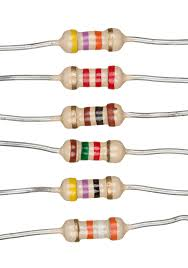
\includegraphics[width=0.6\textwidth]{resistor}
    % Diagram showing the symbol and internal structure of a resistor
    \caption{Symbol and structure of a resistor}
    \label{fig:resistor}
\end{figure}

\begin{figure}[h!]
    \centering
    % 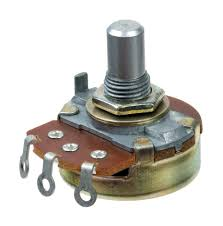
\includegraphics[width=0.6\textwidth]{potentiometer}
    % Diagram showing the symbol and internal structure of a potentiometer
    \caption{Symbol and structure of a potentiometer}
    \label{fig:potentiometer}
\end{figure}

\subsection*{Tables}
\begin{table}[h!]
    \centering
    \caption{Comparison of basic electronic components}
    \label{tab:basic_components}
    \begin{tabular}{|l|l|l|l|}
        \hline
        \textbf{Component} & \textbf{Property} & \textbf{Energy Storage} & \textbf{Common Use} \\
        \hline
        Resistor & Resistance & None & Current limiting, voltage division \\
        Capacitor & Capacitance & Electric field & Energy storage, filtering \\
        Inductor & Inductance & Magnetic field & Energy storage, filtering \\
        \hline
    \end{tabular}
\end{table}

\subsection*{Questions}
\begin{tcolorbox}[colback=gray!10!white,colframe=black!75!black,title={T6A01}]
    What electrical component opposes the flow of current in a DC circuit?
    \begin{enumerate}[label=\Alph*),noitemsep]
        \item Inductor
        \item \textbf{Resistor}
        \item Inverter
        \item Transformer
    \end{enumerate}
\end{tcolorbox}
A resistor opposes the flow of current in a DC circuit, as described by Ohm's Law. Inductors, inverters, and transformers do not primarily oppose current flow in the same way.

%memory_trick T6A01

\begin{tcolorbox}[colback=gray!10!white,colframe=black!75!black,title={T6A02}]
    What type of component is often used as an adjustable volume control?
    \begin{enumerate}[label=\Alph*),noitemsep]
        \item Fixed resistor
        \item Power resistor
        \item \textbf{Potentiometer}
        \item Transformer
    \end{enumerate}
\end{tcolorbox}
A potentiometer is commonly used as an adjustable volume control because it allows for variable resistance, which adjusts the signal level.

%memory_trick T6A02

\begin{tcolorbox}[colback=gray!10!white,colframe=black!75!black,title={T6A03}]
    What electrical parameter is controlled by a potentiometer?
    \begin{enumerate}[label=\Alph*),noitemsep]
        \item Inductance
        \item \textbf{Resistance}
        \item Capacitance
        \item Field strength
    \end{enumerate}
\end{tcolorbox}
A potentiometer controls resistance by adjusting the position of the wiper along the resistive element.

%memory_trick T6A03

\begin{tcolorbox}[colback=gray!10!white,colframe=black!75!black,title={T6A04}]
    What electrical component stores energy in an electric field?
    \begin{enumerate}[label=\Alph*),noitemsep]
        \item Varistor
        \item \textbf{Capacitor}
        \item Inductor
        \item Diode
    \end{enumerate}
\end{tcolorbox}
A capacitor stores energy in an electric field, as opposed to an inductor, which stores energy in a magnetic field.

%memory_trick T6A04

\begin{tcolorbox}[colback=gray!10!white,colframe=black!75!black,title={T6A05}]
    What type of electrical component consists of conductive surfaces separated by an insulator?
    \begin{enumerate}[label=\Alph*),noitemsep]
        \item Resistor
        \item Potentiometer
        \item Oscillator
        \item \textbf{Capacitor}
    \end{enumerate}
\end{tcolorbox}
A capacitor consists of two conductive plates separated by an insulating material (dielectric).

%memory_trick T6A05

\begin{tcolorbox}[colback=gray!10!white,colframe=black!75!black,title={T6A06}]
    What type of electrical component stores energy in a magnetic field?
    \begin{enumerate}[label=\Alph*),noitemsep]
        \item Varistor
        \item Capacitor
        \item \textbf{Inductor}
        \item Diode
    \end{enumerate}
\end{tcolorbox}
An inductor stores energy in a magnetic field, as opposed to a capacitor, which stores energy in an electric field.

%memory_trick T6A06

\begin{tcolorbox}[colback=gray!10!white,colframe=black!75!black,title={T6A07}]
    What electrical component is typically constructed as a coil of wire?
    \begin{enumerate}[label=\Alph*),noitemsep]
        \item Switch
        \item Capacitor
        \item Diode
        \item \textbf{Inductor}
    \end{enumerate}
\end{tcolorbox}
An inductor is typically constructed as a coil of wire, which generates a magnetic field when current flows through it.

%memory_trick T6A07

\begin{tcolorbox}[colback=gray!10!white,colframe=black!75!black,title={T6A08}]
    What is the function of an SPDT switch?
    \begin{enumerate}[label=\Alph*),noitemsep]
        \item A single circuit is opened or closed
        \item Two circuits are opened or closed
        \item \textbf{A single circuit is switched between one of two other circuits}
        \item Two circuits are each switched between one of two other circuits
    \end{enumerate}
\end{tcolorbox}
An SPDT switch connects a single circuit to one of two other circuits, making it useful for routing signals or selecting modes.

%memory_trick T6A08

\subsection*{Summary}
This section covered the basic components used in electronic circuits:
\begin{itemize}
    \item \textbf{Resistors}: Oppose current flow and are used for current limiting and voltage division.
    \item \textbf{Potentiometers}: Adjustable resistors used for volume control and voltage adjustment.
    \item \textbf{Capacitors}: Store energy in an electric field and are used for energy storage and filtering.
    \item \textbf{Inductors}: Store energy in a magnetic field and are used for energy storage and filtering.
    \item \textbf{Switches}: Control the flow of current in circuits, with SPDT switches routing signals between two paths.
\end{itemize}
